%%
%% This is file `mcmthesis-demo.tex',
%% generated with the docstrip utility.
%%
%% The original source files were:
%%
%% mcmthesis.dtx  (with options: `demo')
%% !Mode:: "TeX:UTF-8"
%% -----------------------------------
%%
%% This is a generated file.
%%
%% Copyright (C)
%%     2010 -- 2015 by latexstudio
%%     2014 -- 2016 by Liam Huang
%%
%% This work may be distributed and/or modified under the
%% conditions of the LaTeX Project Public License, either version 1.3
%% of this license or (at your option) any later version.
%% The latest version of this license is in
%%   http://www.latex-project.org/lppl.txt
%% and version 1.3 or later is part of all distributions of LaTeX
%% version 2005/12/01 or later.
%%
%% This work has the LPPL maintenance status `maintained'.
%%
%% The Current Maintainer of this work is Liam Huang.
%%
\documentclass{mcmthesis}
\mcmsetup{CTeX = true,   % 使用 CTeX 套装时,设置为 true
	tcn = 2010225, problem = C,
	sheet = true, titleinsheet = true, keywordsinsheet = true,
	titlepage = false, abstract = true}
\usepackage{palatino}
\usepackage{lipsum}
\usepackage{graphicx}
\usepackage{subfigure} 
\usepackage{float}
\usepackage{caption}
\title{A Wealth of Data}
\begin{document}
	\begin{abstract}
		With the advent of the era of big data, data analysis has become a powerful means of market competition. In this paper, we aim to analyze the sales data of three types of products in the market and user reviews to provide recommendations for the sale of products.
		
		First of all, we analyze the difference in sales between products and the trend of change, which provides us with a direct view of the market situation.
		
		Second, we perform word frequency statistics on user evaluations and use the results after removing stopwords as the basis for subsequent analysis.
		
		Third, in word frequency statistics, we noticed that some words are related to the nature of the product. Statistics for these words are critical to improving a product or launching a new product.
		
		Fourth, many words express user emotions in user reviews. These words have a lot to do with their star ratings.
		
		Fifth, we analyzed the relationship between the star ratings of previous users and the reviews over some time.
		
		Sixth, through the processing of natural language, we rate each comment according to its sentiment. We also compare scores with the user's star ratings to verify their accuracy.
		
		Finally, we combined data from product sales records and user reviews to identify a way to measure products.
		\begin{keywords}
			keyword1; keyword2
		\end{keywords}
	\end{abstract}
	\maketitle
	\section{Introduction}
	
	\subsection{Background}
	
	
	\subsection{Program Restatement}
	
	\subsection{Solution Introduction}
	
	\section{Data Processing and Conclusion Analysing}
	
	\subsection{Sales-Based Analysis}
	We screened sales data for three types of products, and selected the three products with the highest sales volume to draw sales-time line charts. The results are as follows.
	
	\begin{figure}[H]
		\small
		\centering
		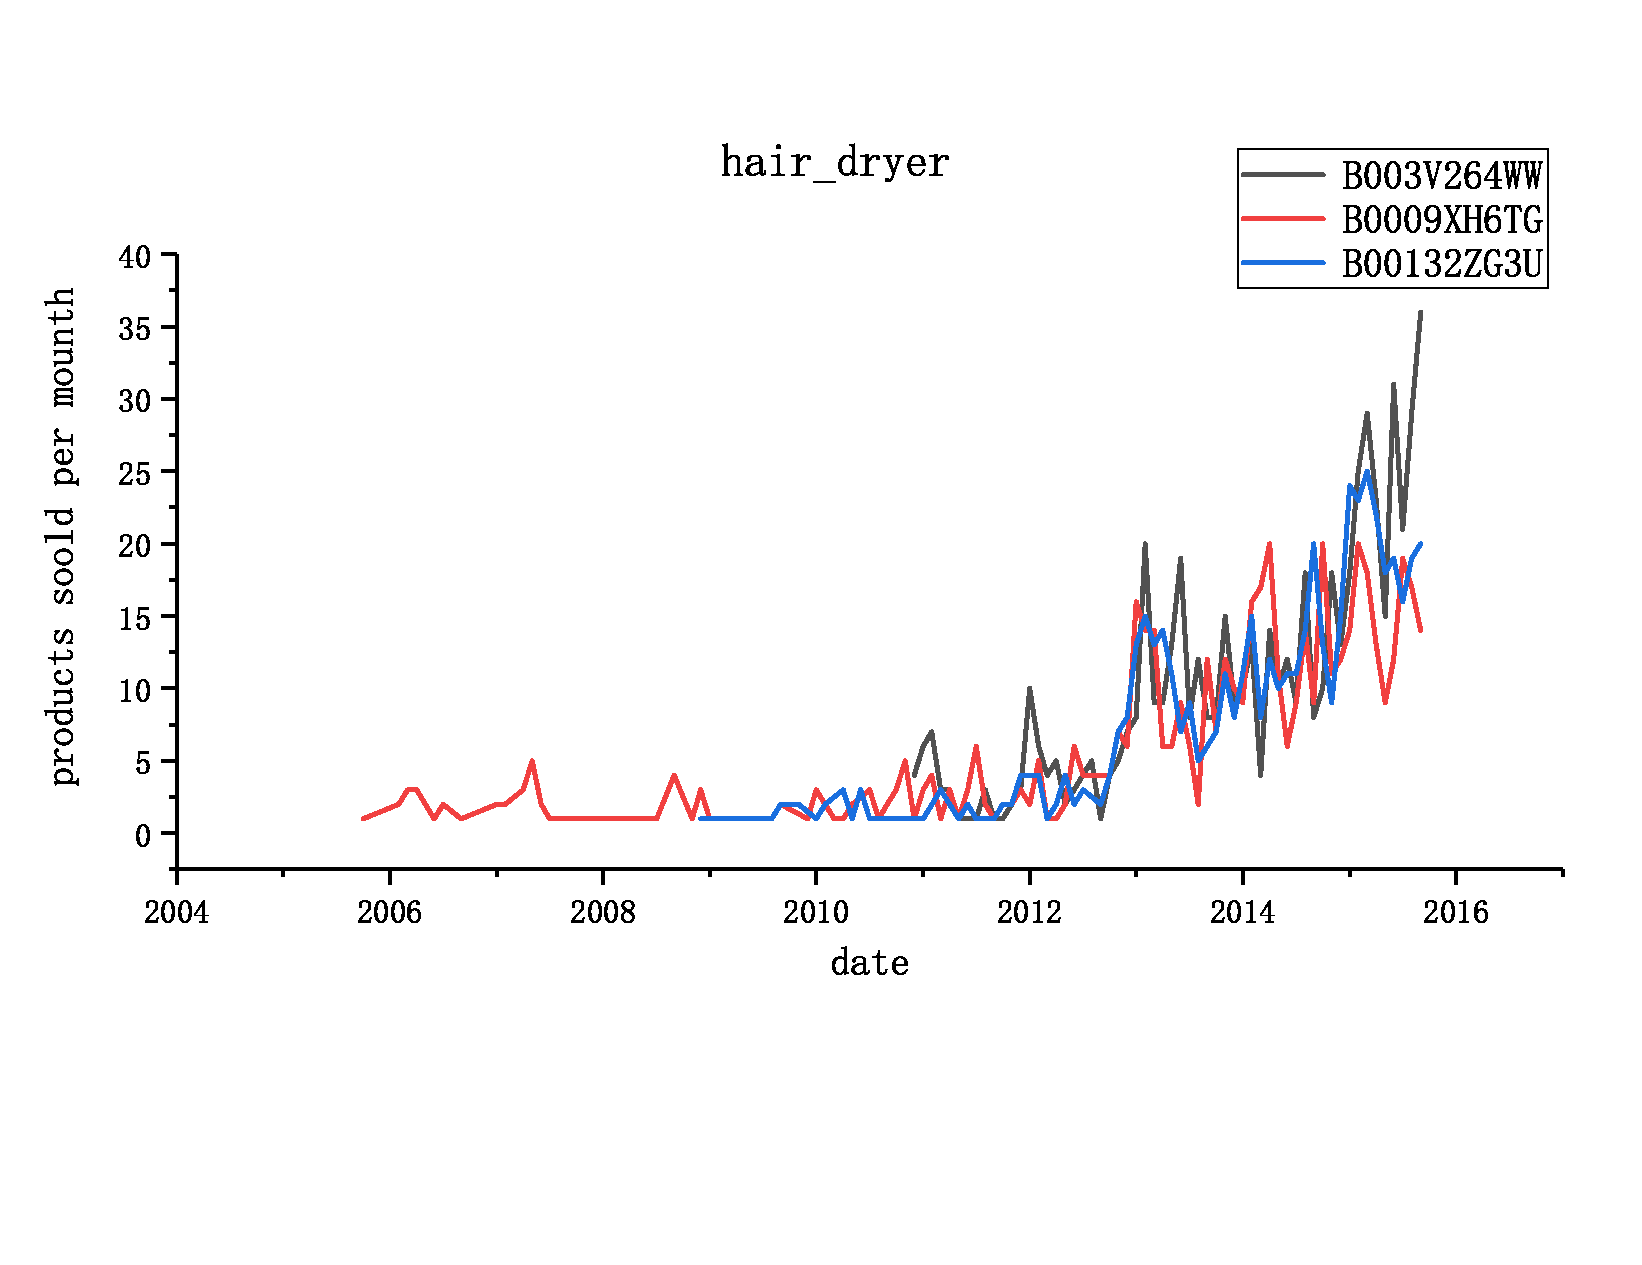
\includegraphics[width=13cm]{hair_dryer.eps}
		\caption{hair dryer sales} \label{hair dryer sales}
	\end{figure}
	
	\begin{figure}[H]
		\small
		\centering
		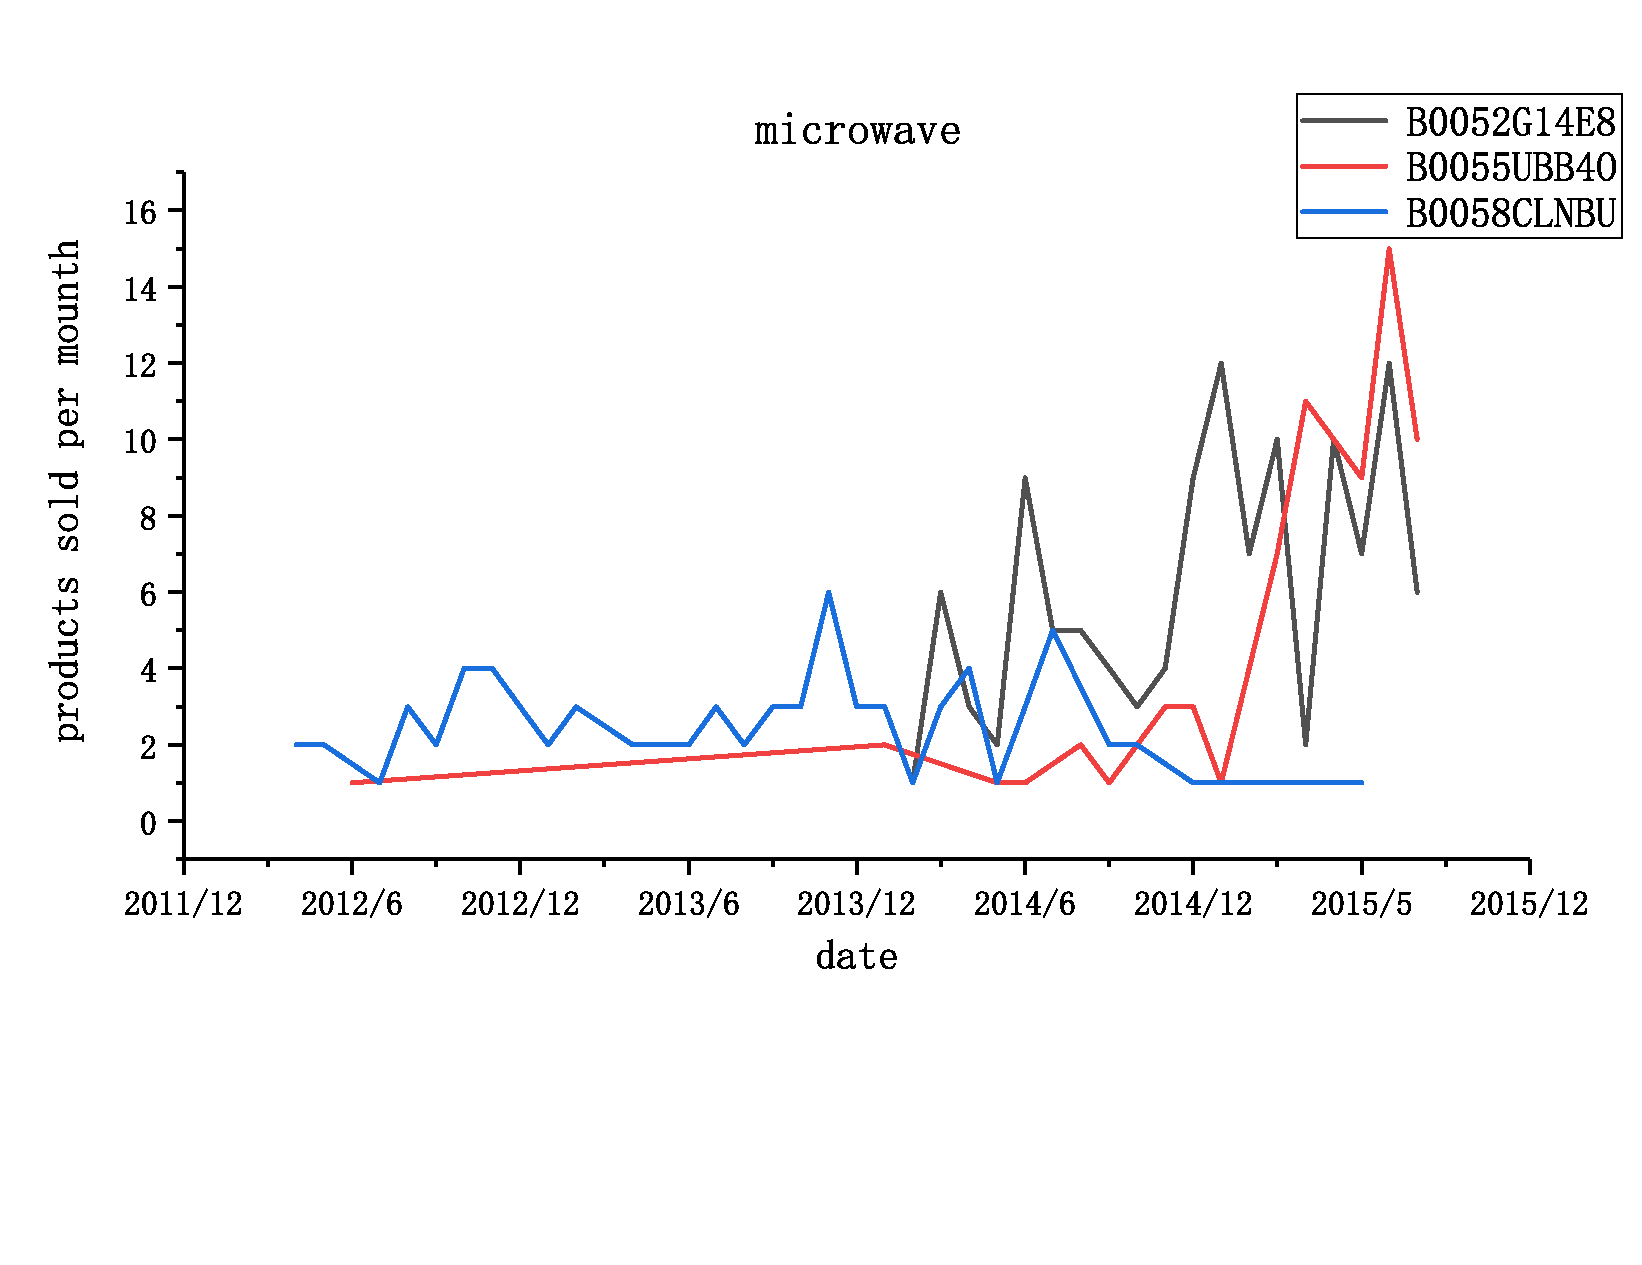
\includegraphics[width=13cm]{microwave.eps}
		\caption{microwave sales} \label{microwave sales}
	\end{figure}
	
	\begin{figure}[H]
		\small
		\centering
		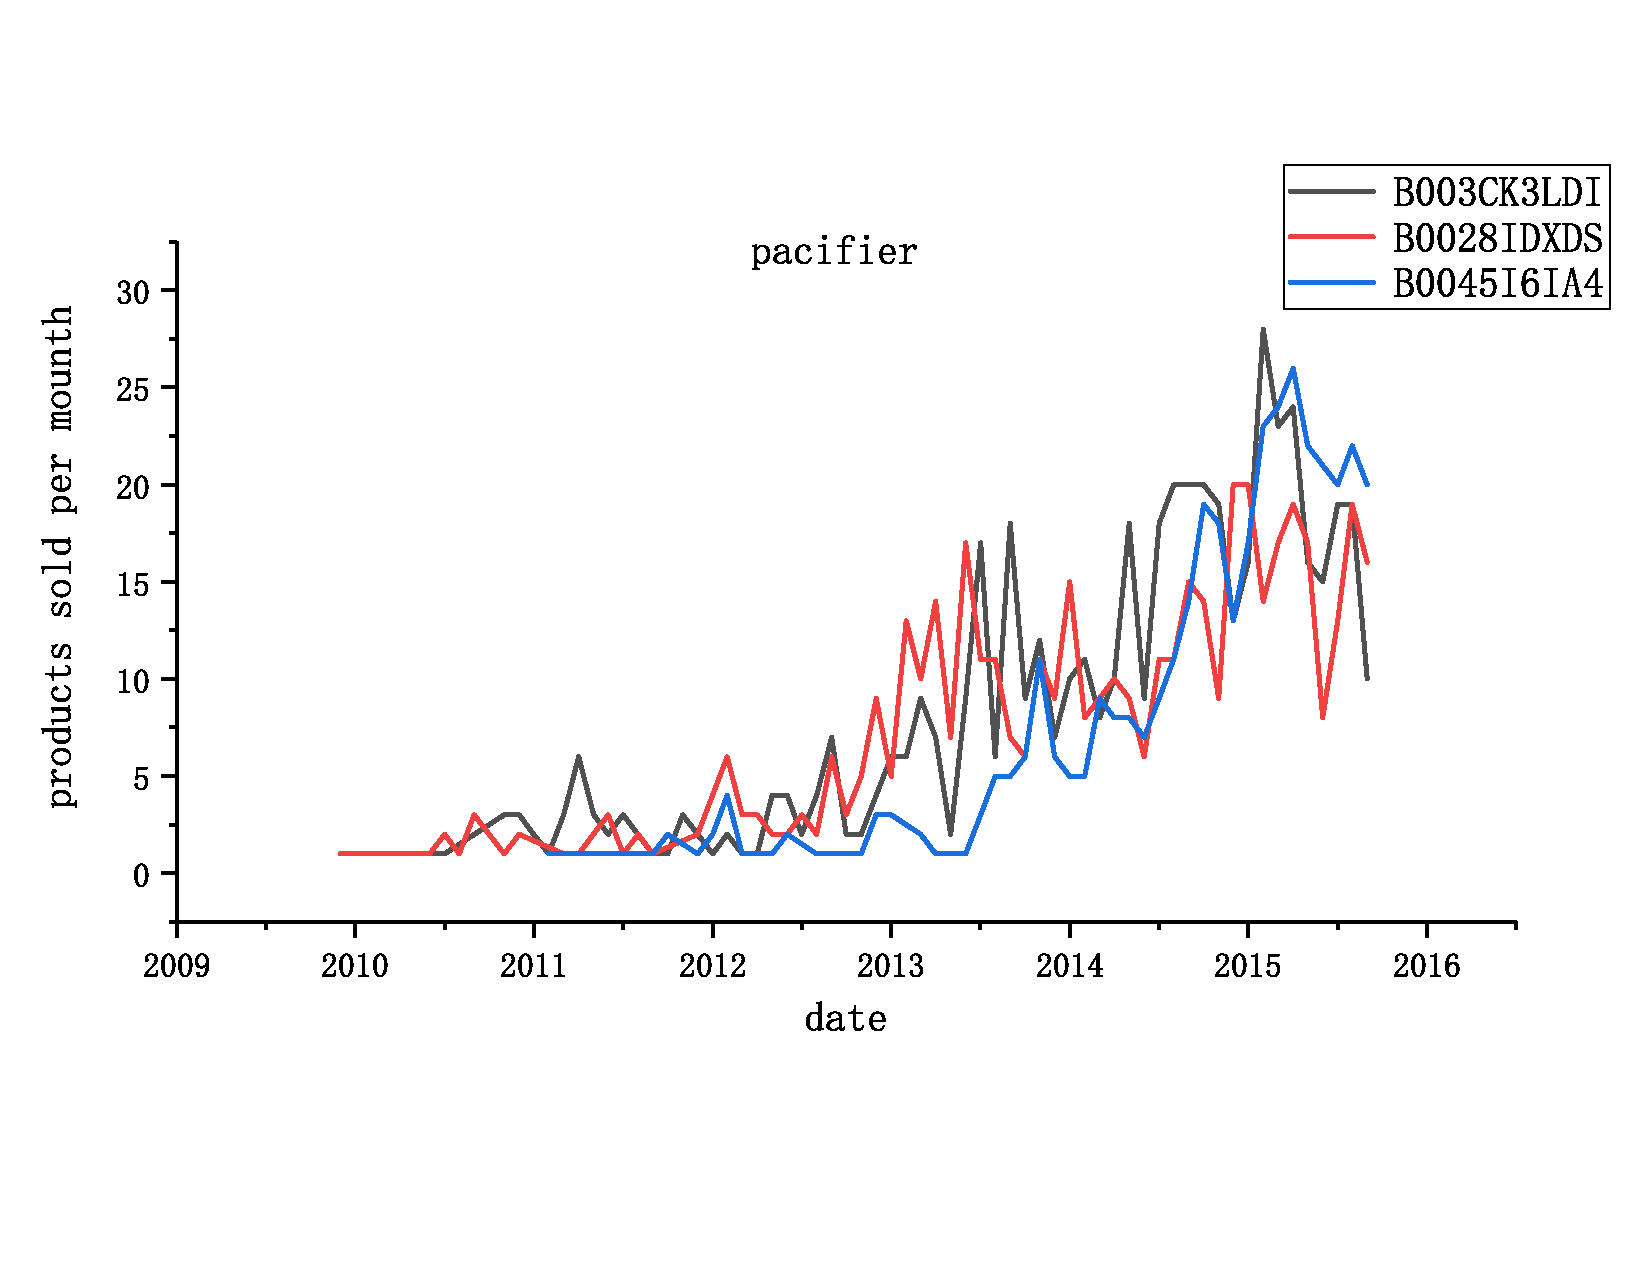
\includegraphics[width=13cm]{pacifier.eps}
		\caption{pacifier sales} \label{pacifier sales}
	\end{figure}
	
	By simply analyzing these images, we have reached some conclusions:
	\begin{itemize}
		\item
		The total sales of the three products are significantly different. The sales of hair dryers and pacifiers are much larger than microwave ovens, and the market competition is more intense.
		\item
		For hair dryers, some products have been sold early, but their sales have grown slowly. Other products have only begun to appear in recent years, but sales have grown rapidly, quickly surpassing older products. The total sales volume of hair dryers has increased rapidly in recent years and has great market potential.
		\item
		The overall sales of the microwave oven market are low with relatively large fluctuations. Some products maintain low monthly sales and still have a downward trend. Some new products have good sales as soon as they hit the market. This may be because buyers of microwave ovens value new features of the products more.
		\item
		The sales of pacifiers are also generally increasing, but most of the best-selling products have a long sales history. This may be because for products such as pacifiers, people prefer products that are safe and reliable, and are more willing to choose a brand that sells well and is well received.
	\end{itemize}
	
	However, sales-based analysis is not enough. Below we will analyze the data from some other angles.
	
	\subsection{Count the Word Frequency Statistics}
	To analyze the review of consumers, we divided the review into high score (3-4 points) and a low score (1-2 points). First of all, we synthesize the reviews of the three products and find out the word frequency. Then we deal with the high-grade reviews and low-grade reviews of the three products respectively. The python code is attached. For the python code, see the appendix.
	\subsubsection{Remove Stopwords}
	Because some commonly used words are used quite frequently, such as a the, he, etc. in English, almost all comments contain these words. If they are used as keywords, almost all comments will be indexed, and there is no differentiation, so these words are generally removed directly, not as keywords.
	
	
	\subsection{Advantages and Disadvantages of Three Products}
	After the word frequency is counted and the stop words are removed, the reason why people like/dislike the product is obtained by analyzing the words with high word frequency.
	By counting the number of times that people mentioned the reason, we summed up 5 factors of success or failure of these products.
	\subsubsection{Pacifier}
	\begin{figure}[H]
		\begin{minipage}[t]{0.5\textwidth}
			\centering
			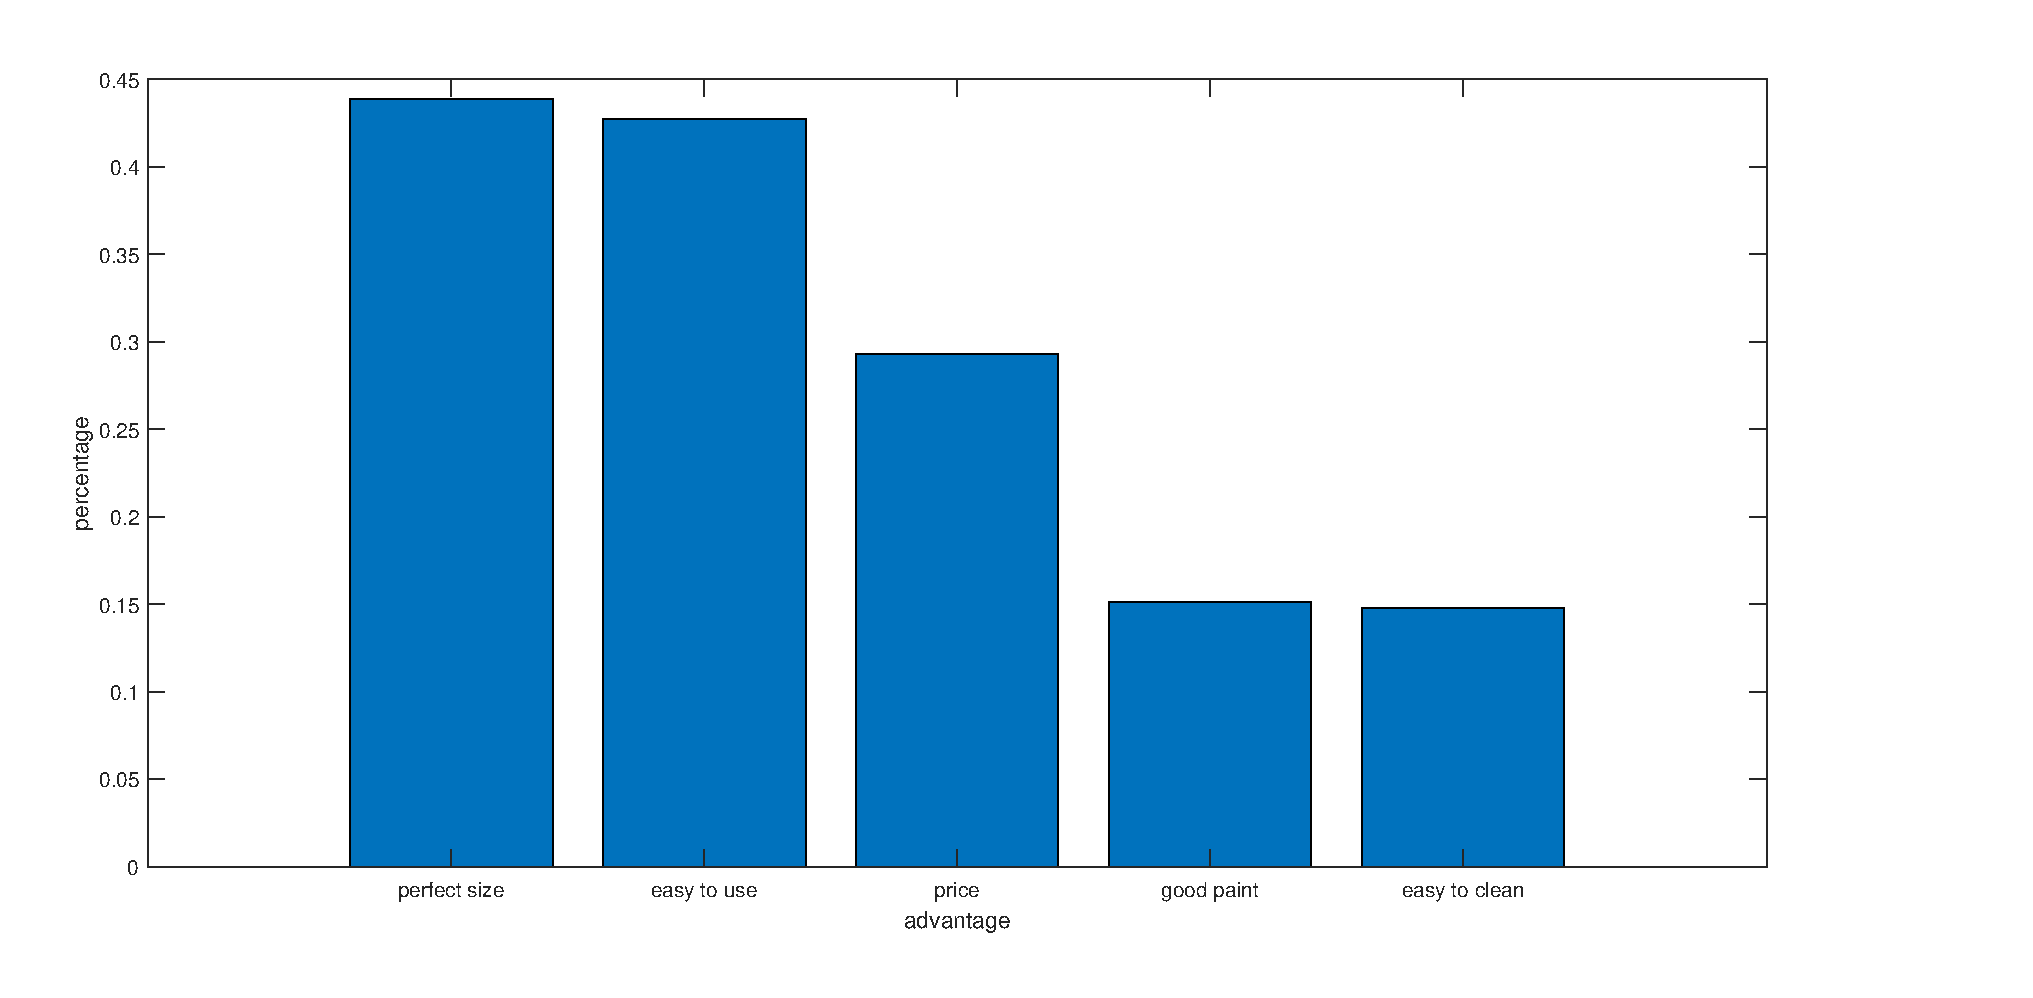
\includegraphics[scale=0.5]{pacifier_advantage.eps}
			\caption{The proportion of reasons people like the pacifier\label{fig:1}}
		\end{minipage}
		\qquad
		\begin{minipage}[t]{0.5\textwidth}
			\centering
			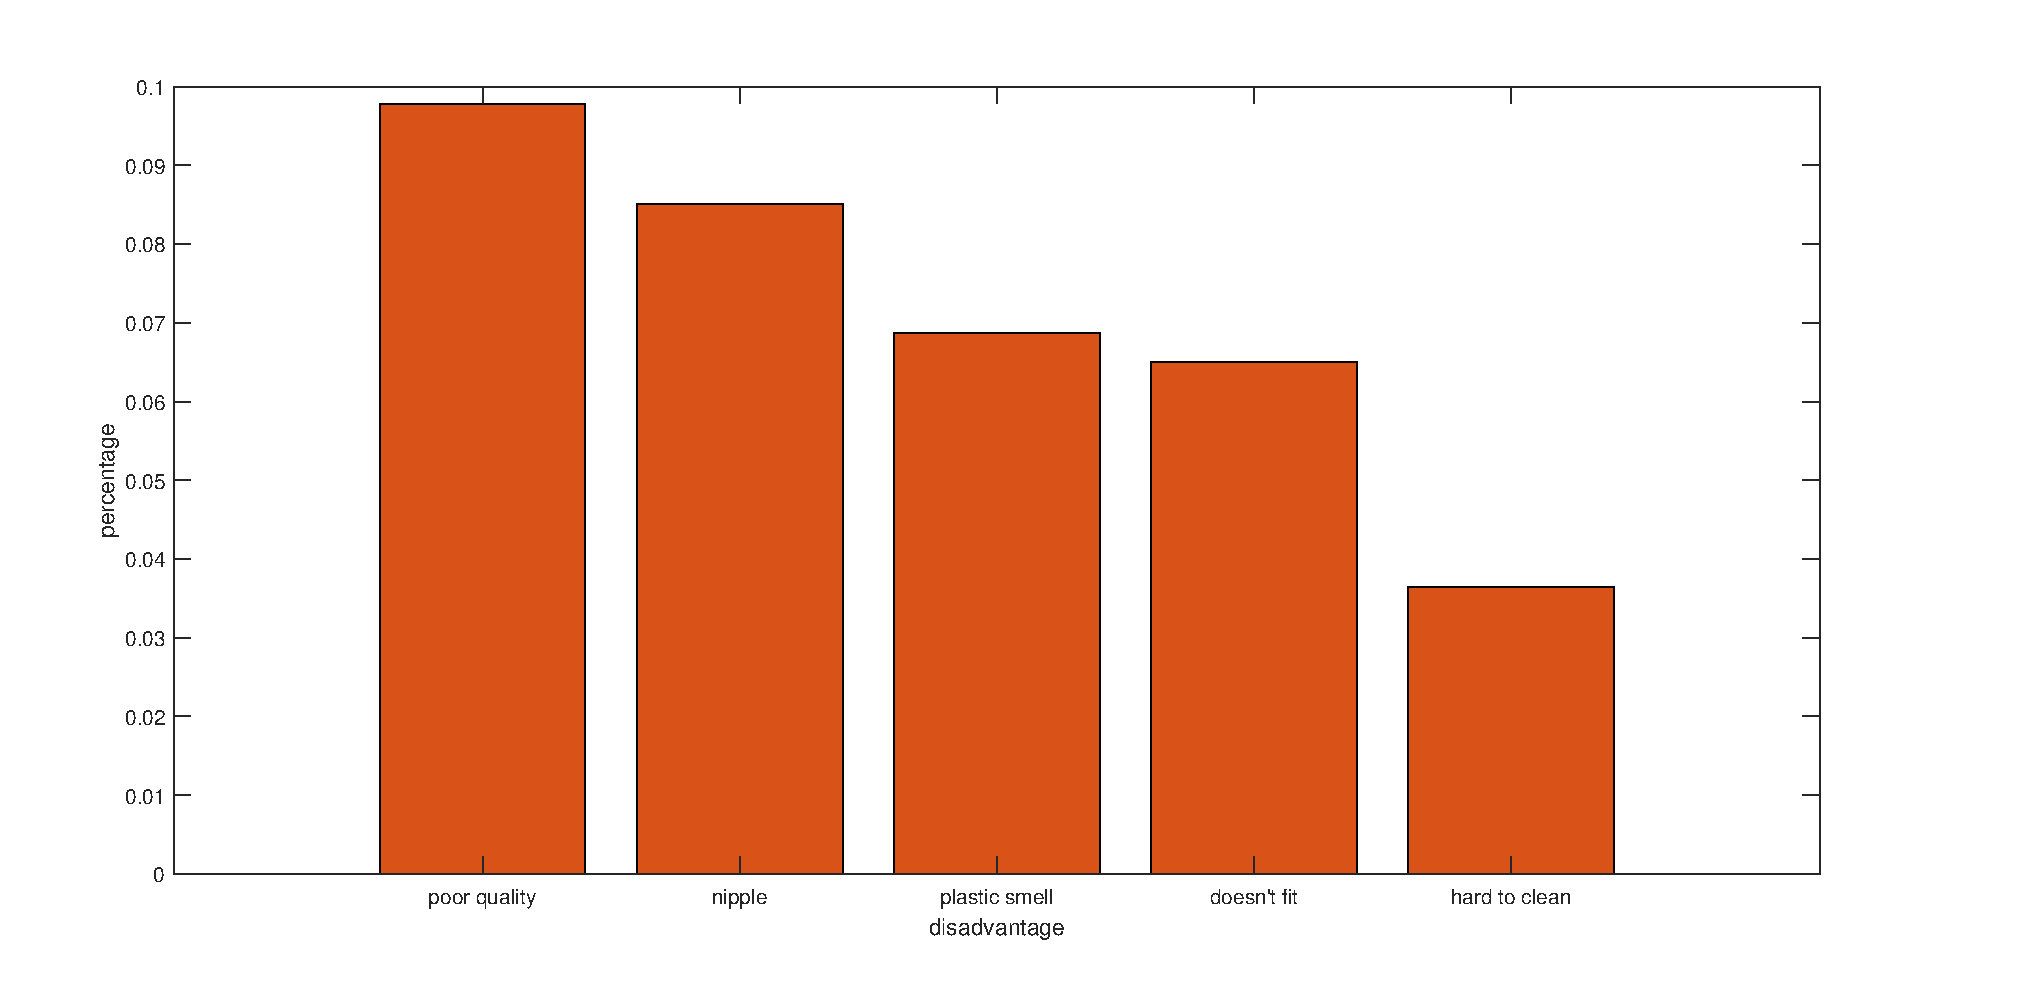
\includegraphics[scale=0.5]{pacifier_disadvantage.eps}
			\caption{The proportion of reasons people dislike the pacifier\label{fig:2}}
		\end{minipage}
	\end{figure}
	\begin{flushleft}
		As shown in the chart, ease of use is the most outstanding advantage of the product. About 17\% of high scoring customers mentioned this feature in their comments. After that is cute, quality, price and pacifier design.
		
	\end{flushleft}
	\begin{flushleft}
		On the other hand, about 9.5\% of people who don't like the product complain
		about the poor quality. Although 4\% of people who like the product think that the nipple fits well with there baby's mouth, 7\%  think that the nipple leaks, or is too short and hard. Besides, people can't bear the plastic smell, which is an important reason why they don't like it. Furthermore, some parents think that the pacifier doesn't fit well. At last, about 3\% of people find it hard to clean the pacifier, which makes them give low ratings.
	\end{flushleft}
	
	
	\subsubsection{Hair Dryer}
	\begin{figure}[H]
		\begin{minipage}[t]{0.5\textwidth}
			\centering
			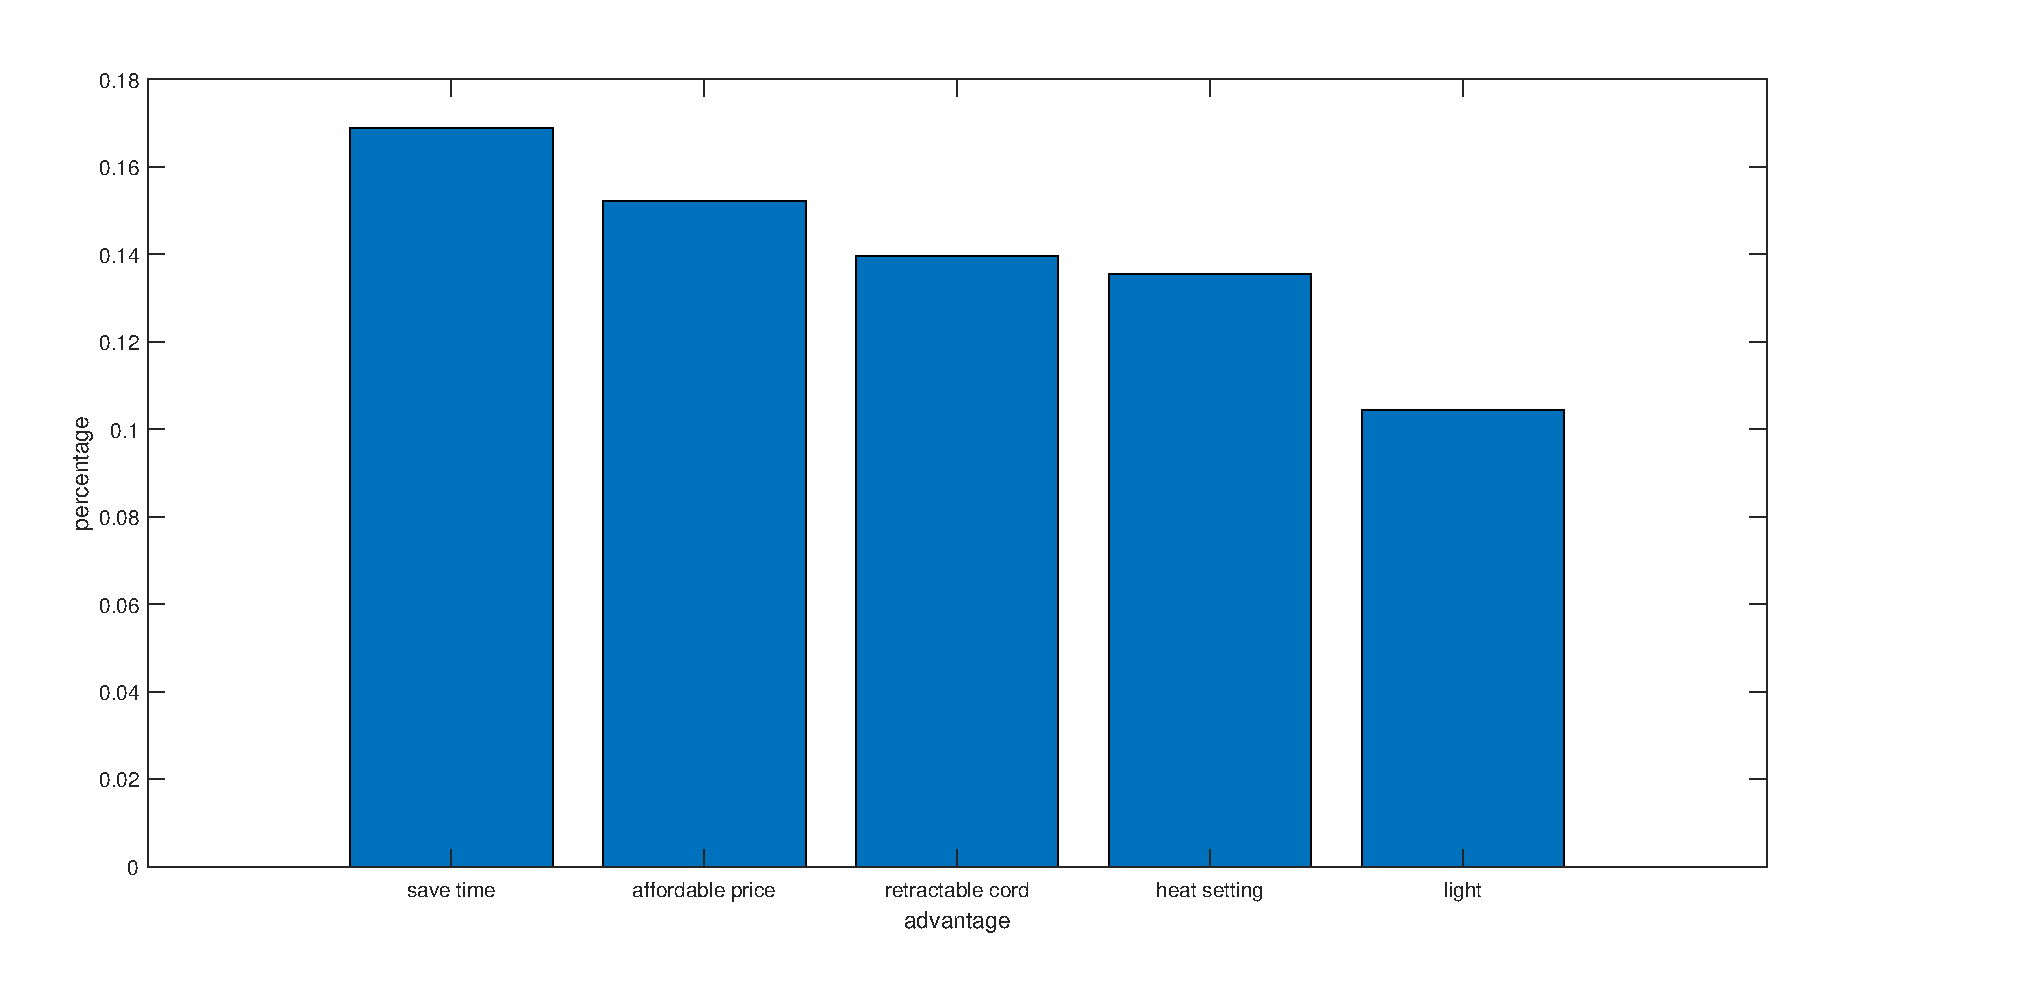
\includegraphics[scale=0.5]{hair_dryer_advantage.eps}
			\caption{The proportion of reasons people like the hair dryer}
		\end{minipage}
		\qquad
		\begin{minipage}[t]{0.5\textwidth}
			\centering
			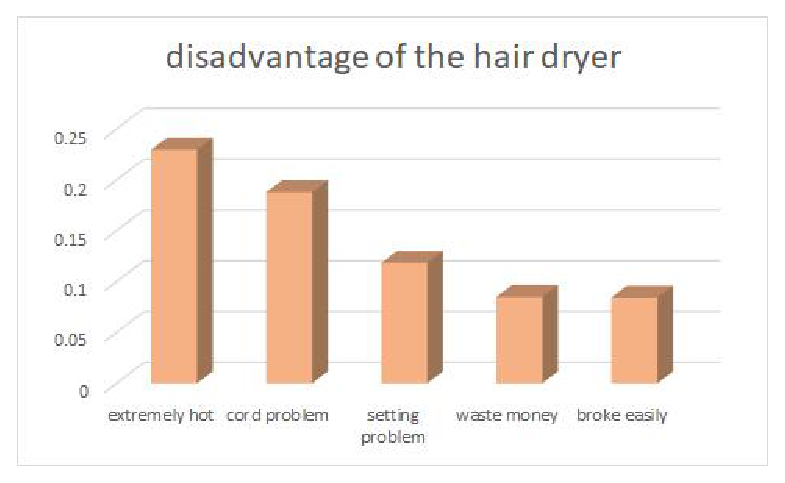
\includegraphics[scale=0.5]{hair_dryer_disadvantage.eps}
			\caption{The proportion of reasons people dislike the hair dryer }
		\end{minipage}
	\end{figure}
	\begin{flushleft}
		According to the figure,16\% of people think it saves their time, while 14\% were attracted by the affordable price.12\% think the retractable cord is a good design. Besides, the hairdryer is light to carry, so 10\% of customers give a high rating. At last, the heating setting design is also attractive.
	\end{flushleft}
	\begin{flushleft}
		From the figure, we can know that about 21\% of people can't stand the extreme hot of the hair dryer.17\% complained that the cord broke quickly.10\% find that the setting mode has some problem.7\% think buying the hairdryer is a waste of money, and the same percentage of people wrote that the hairdryer broke quickly.
	\end{flushleft}
	
	\subsubsection{Microwave}
	\begin{figure}[H]
		\begin{minipage}[t]{0.5\textwidth}
			\centering
			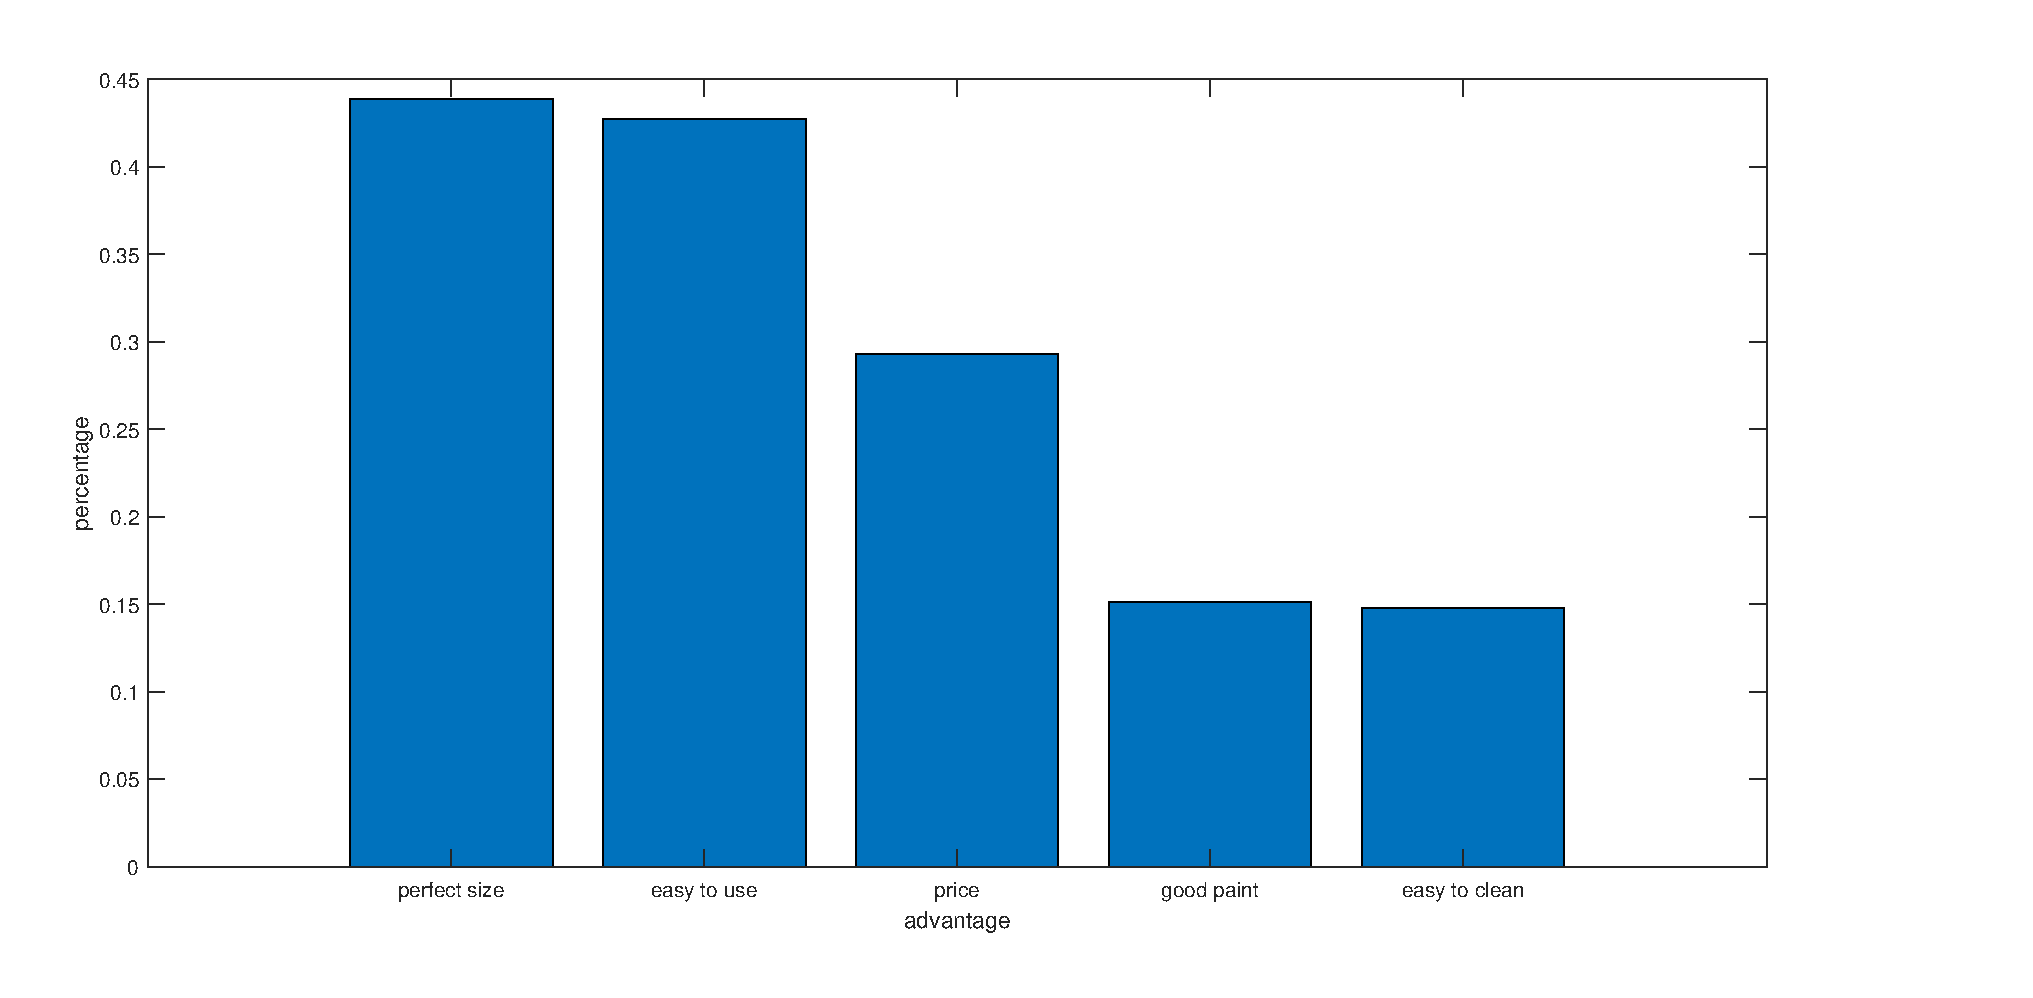
\includegraphics[scale=0.5]{microwave_advantage.eps}
			\caption{The proportion of reasons people like the microwave\label{fig:1}}
		\end{minipage}
		\qquad
		\begin{minipage}[t]{0.5\textwidth}
			\centering
			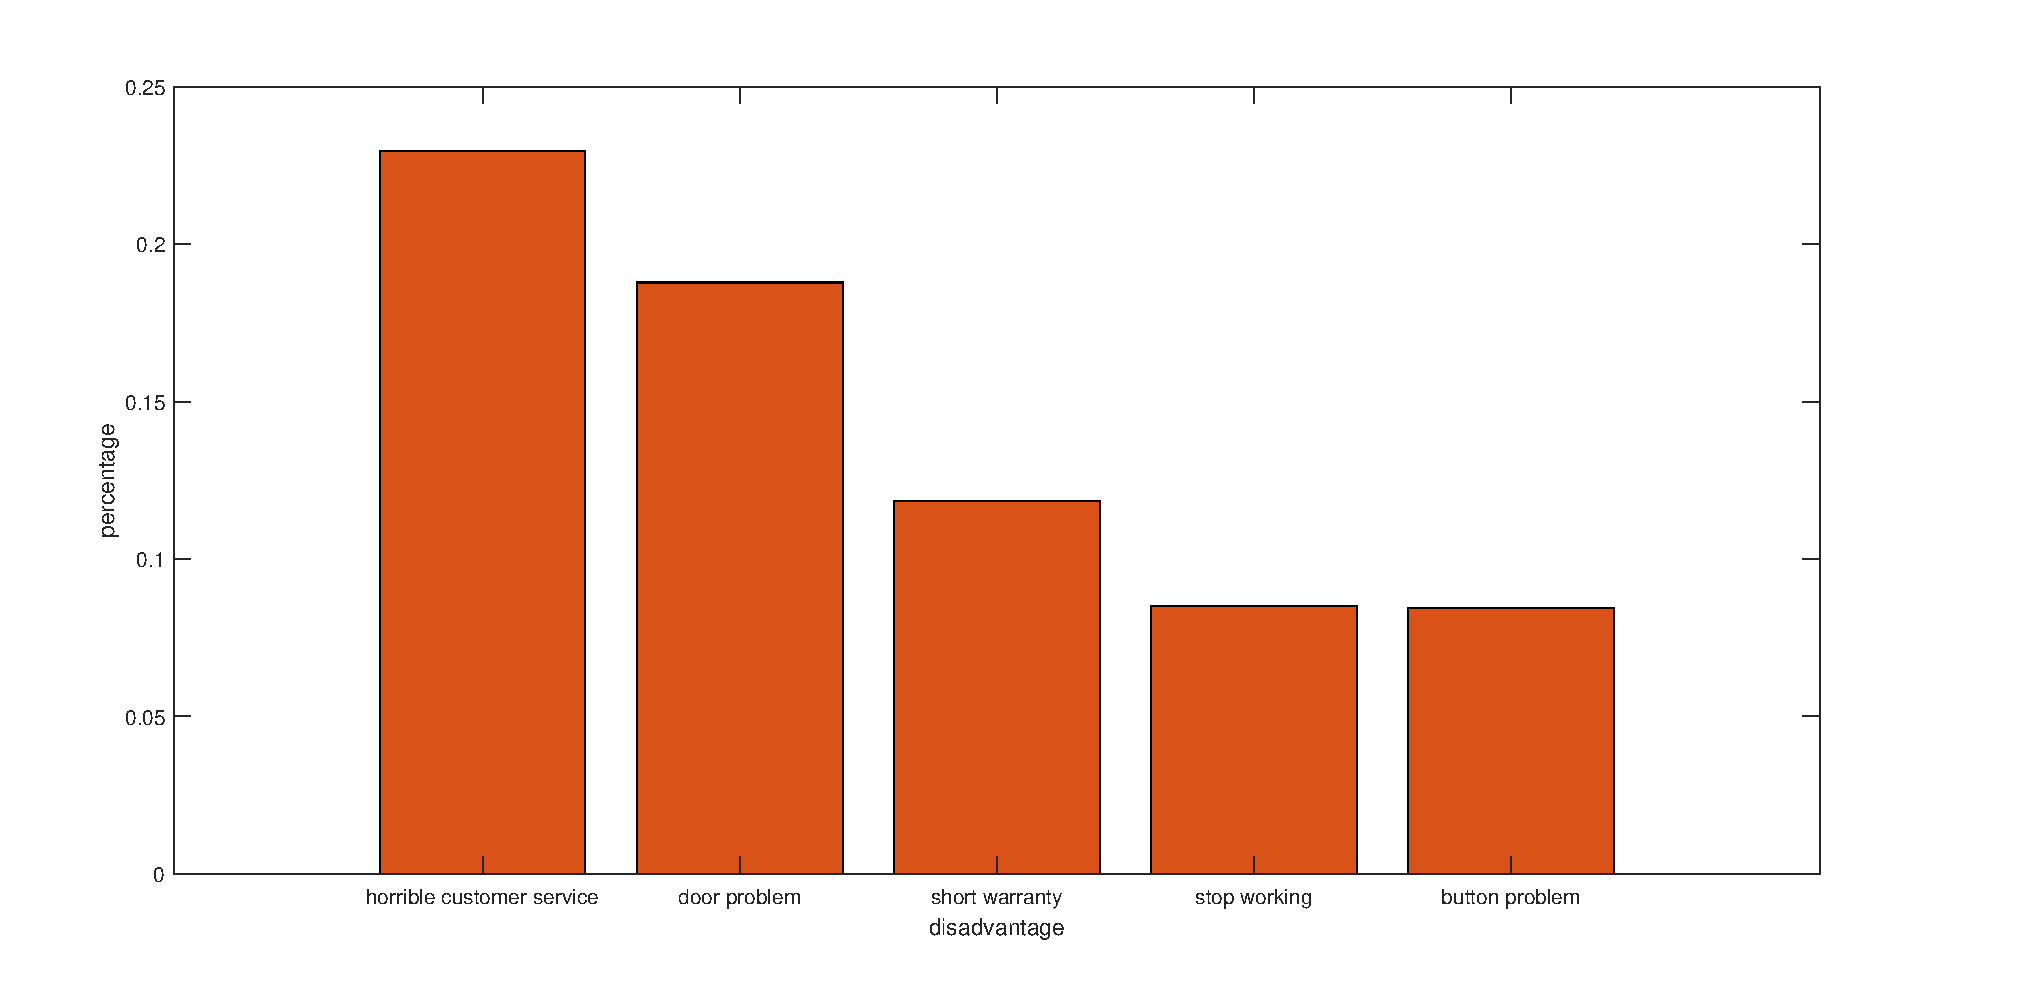
\includegraphics[scale=0.5]{microwave_disadvantage.eps}
			\caption{The proportion of reasons people dislike the microwave\label{fig:2}}
		\end{minipage}
	\end{figure}
	\begin{flushleft}
		About 35\% of customers love its size. They said they can put it anywhere in the kitchen and it fits well.21\% thinks it's easy to use.15\% people think that the price is fair.
		6\% enjoy its paint. And some other people find the microwave easy to clean.
	\end{flushleft}
	\begin{flushleft}
		However, problems still exist. Customers complain that the customer service is horrible. Besides, the door of the microwave has many problems. Furthermore,20\% think warranty time is too short. About 9\% of people said that their microwave stop working or the button broke;
	\end{flushleft}
	
	
	\subsection{Relations between Specific Quality Descriptors and Rating Levels}
	We choose 8 specific quality descriptors. And their frequency is shown in the table.
	\begin{table}[H]
		\centering
		\caption{The number of times the word was mentioned}
		\begin{tabular}{|c|c|c|c|c|c|c|c|c|}
			\hline 
			& love & perfect & nice & cute & disappointed & waste & bad & junk \\ 
			\hline 
			high rating & 8193 & 2591 & 2483 & 2435 & 165 & 65 & 339 & 20 \\ 
			\hline 
			low rating & 187 & 64 & 185 & 189 & 432 & 292 & 260 & 149 \\ 
			\hline 
		\end{tabular}
	\end{table}
	
	We calculated the probability of these words appearing in high rating reviews and low rating reviews, respectively.
	
	\begin{align}
	p(word\_in\_high\_rating)=\frac{\frac{num\_in\_high}{high\_num}}
	{\frac{num\_in\_high}{high\_num}+\frac{num\_in\_low}{low\_num}}
	\end{align}
	\begin{flushleft}
		\begin{itemize}
			\item  $word\_in\_high\_rating$:Probability of words appearing in high scoring comments 
			\item	$num\_in\_high$ :The number of times words appear in high rated comments
			\item $num\_in\_low$ :The number of times words appear in low rated comments
			\item $high\_num$ :Number of high rated comments
			\item $low\_num$ :Number of low rated comments
		\end{itemize}
	\end{flushleft}
	
	\begin{figure}[H]
		\begin{minipage}[t]{1\textwidth}
			\centering
			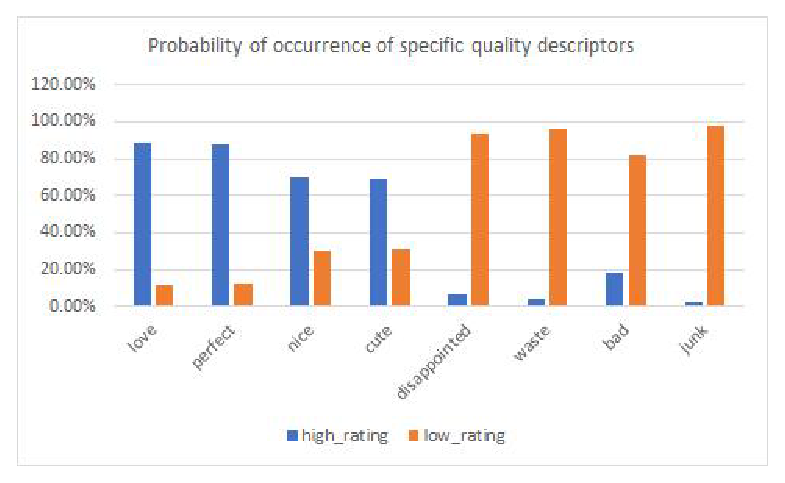
\includegraphics[scale=1]{total.eps}
			\caption{probability the word appear in high/low rating comments\label{fig:1}}
		\end{minipage}
	\end{figure}
	\begin{flushleft}
		As we can see, if the word 'love' or 'perfect' appears in the review, Users nearly have a 90\% chance to give high scores. On the contrary, if the word 'disappointed' is in the review, We can almost conclude that the user will give a low rating.
	\end{flushleft}
	So it is obvious that specific quality descriptors are strongly associated with rating levels.
	
	\subsection{Do specific star ratings incite more reviews? }
	\subsubsection{Theory}
	
	To analyze whether some specific star ratings lead to more reviews, we have analyzed the highest selling products for hair dryers, microwave ovens, and pacifiers. First, we counted the number of reviews per month for a certain product and the number of reviews per month for five ratings of the product and then used the correlation coefficient formula to calculate the correlation coefficient between the total number of reviews and a certain number of star ratings. The correlation coefficients corresponding to the scores are compared. When a certain correlation coefficient is large, the more the certain star ratings in a certain period, the more the user's comments will be. That is to say, the number of certain star ratings and the total number of star ratings are in a linear relationship. That way, we have every reason to believe that this rating will incite more reviews.
	
	\subsubsection{Data Processing}
	
	Here is the table of the correlation coefficient for every star rating:
	
	% Please add the following required packages to your document preamble:
	% \usepackage{graphicx}
	\begin{table}[H]
		\centering
		\caption{correlation coefficient for every star rating}
		\resizebox{\textwidth}{!}
		{%
			\begin{tabular}{|l|l|l|l|l|l|}
				\hline
				product    & star1 & star2 & star3 & star4 & star5 \\ \hline
				hair dryer & 0.68  & 0.46  & 0.69  & 0.85  & 0.97  \\ \hline
				microwave  & 0.58  & 0.38  & 0.6   & 0.57  & 0.72  \\ \hline
				pacifier   & 0.35  & 0.36  & 0.5   & 0.61  & 0.98  \\ \hline
			\end{tabular}%
		}
	\end{table}
	
	Here is the graph based on the above table:
	
	\begin{figure}[H]
		\small
		\centering
		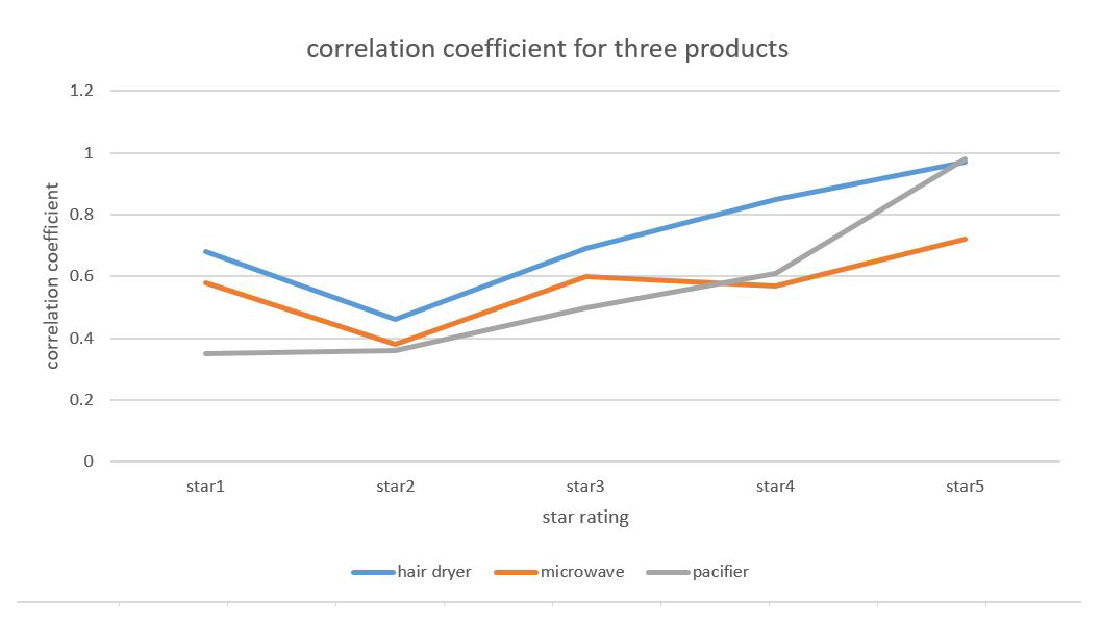
\includegraphics[width=15cm]{correlation coefficient incite.eps}
		\caption{correlation coefficient incite} \label{fig:correlation coefficient incite}
	\end{figure}
	
	\subsubsection{Conclusion}
	
	As can be seen from the above chart, the correlation coefficient with a star of 5 is the largest. This means that a 5-star rating will lead to more reviews.
	
	\subsection{Using DNN to Calculate the Value of the Reviews}
	The emotion analysis system is one of the most classical applications in natural language processing. We use the algorithm developed by Han Xiao and Yao Lu\cite{1} to map the degree of whether a customer likes or dislikes the product to the range of [0,1], to quantitatively reflect the attitude expressed by the comment.
	\subsubsection{Preprocessing}
	
	
	The original text data often has many parts that affect the final classification effect. This part of data or text needs to be cleaned at the beginning of text classification, otherwise, it will easily lead to the so-called "trash in, trash out" problem\cite{2}
	
	In addition to the steps of missing value processing, de-duplication processing and noise processing included in the data cleaning of general classification problems, we also clean up the following data:
	\begin{itemize}
		\item Non-text data: HTML tags, URL addresses, and other non-text content are often attached to the text, so it is necessary to clear this part of the content that is not helpful for classification.
		\item Meaningless text: Besides, the rest of the text, such as advertising content, copyright information, and personal signature, should also be filtered out, which should not be learned as features.
	\end{itemize}
	\subsubsection{Algorithm}
	In the algorithm,Dynamic Convolution Neural Network is used as the sentiment prediction algorithm.The network layers are set as follows:
	\begin{itemize}
		\item Embedding layer: set as the lowest layer, to get the vector representation for individual words to form the matrix representation of the sentence
		\item Convolutional Layer: extracts local features by performing 2d convolution on the sentence matrix
		\item K-max pooling layer: extracts kth strongest signals on a per-feature basis
		\item Folding layer: adds interaction among features by "folding" the input matrix
		\item Logistic regression layer: the final layer that makes the prediction by assigning scores to each output label
	\end{itemize}
	
	
	\subsection{Verifying the Accuracy of Review-Based Ratings}
	In the previous subsection, we analyzed reviews using natural language processing and gave a score for each record. This subsection we will verify the accuracy of the previously given score.
	
	We believe that the correlation coefficient between review-based ratings and star ratings can well reflect the accuracy of the reviews analysis. In order to calculate the correlation coefficient, we need to first calculate the covariance of these two data.Covariance can be easily calculated by the following equation:
	$$Cov(X,Y)=E[(X-E[X])(Y-E[Y])]$$
	Cov (X, Y) represents the covariance of X and Y, and E (X) represents the expectation of X.
	
	After getting the covariance, we used the following formula to calculate the correlation coefficient:
	$$r(X,Y)=\frac{Cov(X,Y)}{\sqrt{Var[X]Var[Y]}}$$
	Here r (X, Y) represents the correlation coefficient between X and Y, and Var [X] represents the variance of X.
	
	We calculated the total correlation coefficients of the three categories of products, and the correlation coefficients of high star rating (4-5) and low star rating (1-2). The results are as follows:
	
	
	
	\begin{table}[h]
		\begin{center} 
			\caption{correlation coefficient between review-based ratings and star ratings}
			\begin{tabular}{|c|c|c|}
				\hline
				&                  & correlation coefficient \\ \hline
				\multirow{3}{*}{hair dryer}     & high star rating & 0.4201                  \\ \cline{2-3} 
				& low star rating  & 0.4934                  \\ \cline{2-3} 
				& all              & 0.5964                  \\ \hline
				\multirow{3}{*}{microwave oven} & high star rating & 0.3978                  \\ \cline{2-3} 
				& low star rating  & 0.5381                  \\ \cline{2-3} 
				& all              & 0.6753                  \\ \hline
				\multirow{3}{*}{baby pacifier}  & high star rating & 0.4372                  \\ \cline{2-3} 
				& low star rating  & 0.4557                  \\ \cline{2-3} 
				& all              & 0.5797                  \\ \hline
			\end{tabular}
		\end{center}
	\end{table}
	
	
	As can be seen from the table, review-based ratings are positively related to star rating satisfaction. In the case where the review-based score is relatively low, especially when the star rating is in the middle level, the correlation coefficient is relatively high. Overall our review-based ratings are acceptable.
	
	
	\subsection{User Evaluation}
	\subsubsection{Theory}
	To get a user evaluation of the top three hair dryers, microwaves, and pacifiers, we came up with the following measurement method. To make full use of reviews and ratings, we combined text-based ratings and star-based ratings, each giving different weights, and finally got a most informative measure. The formula is as follows:
	$$
	average\ rating = 0.8 \times star\_rating + text\_rating
	$$
	
	\subsubsection{Data Processing}
	
	First of all, let's see the chart of the top three hair dryers\ (product\_id: B003V264WW, B0009XH6TG, B00132ZG3U):
	
	\begin{figure}[H]
		\small
		\centering
		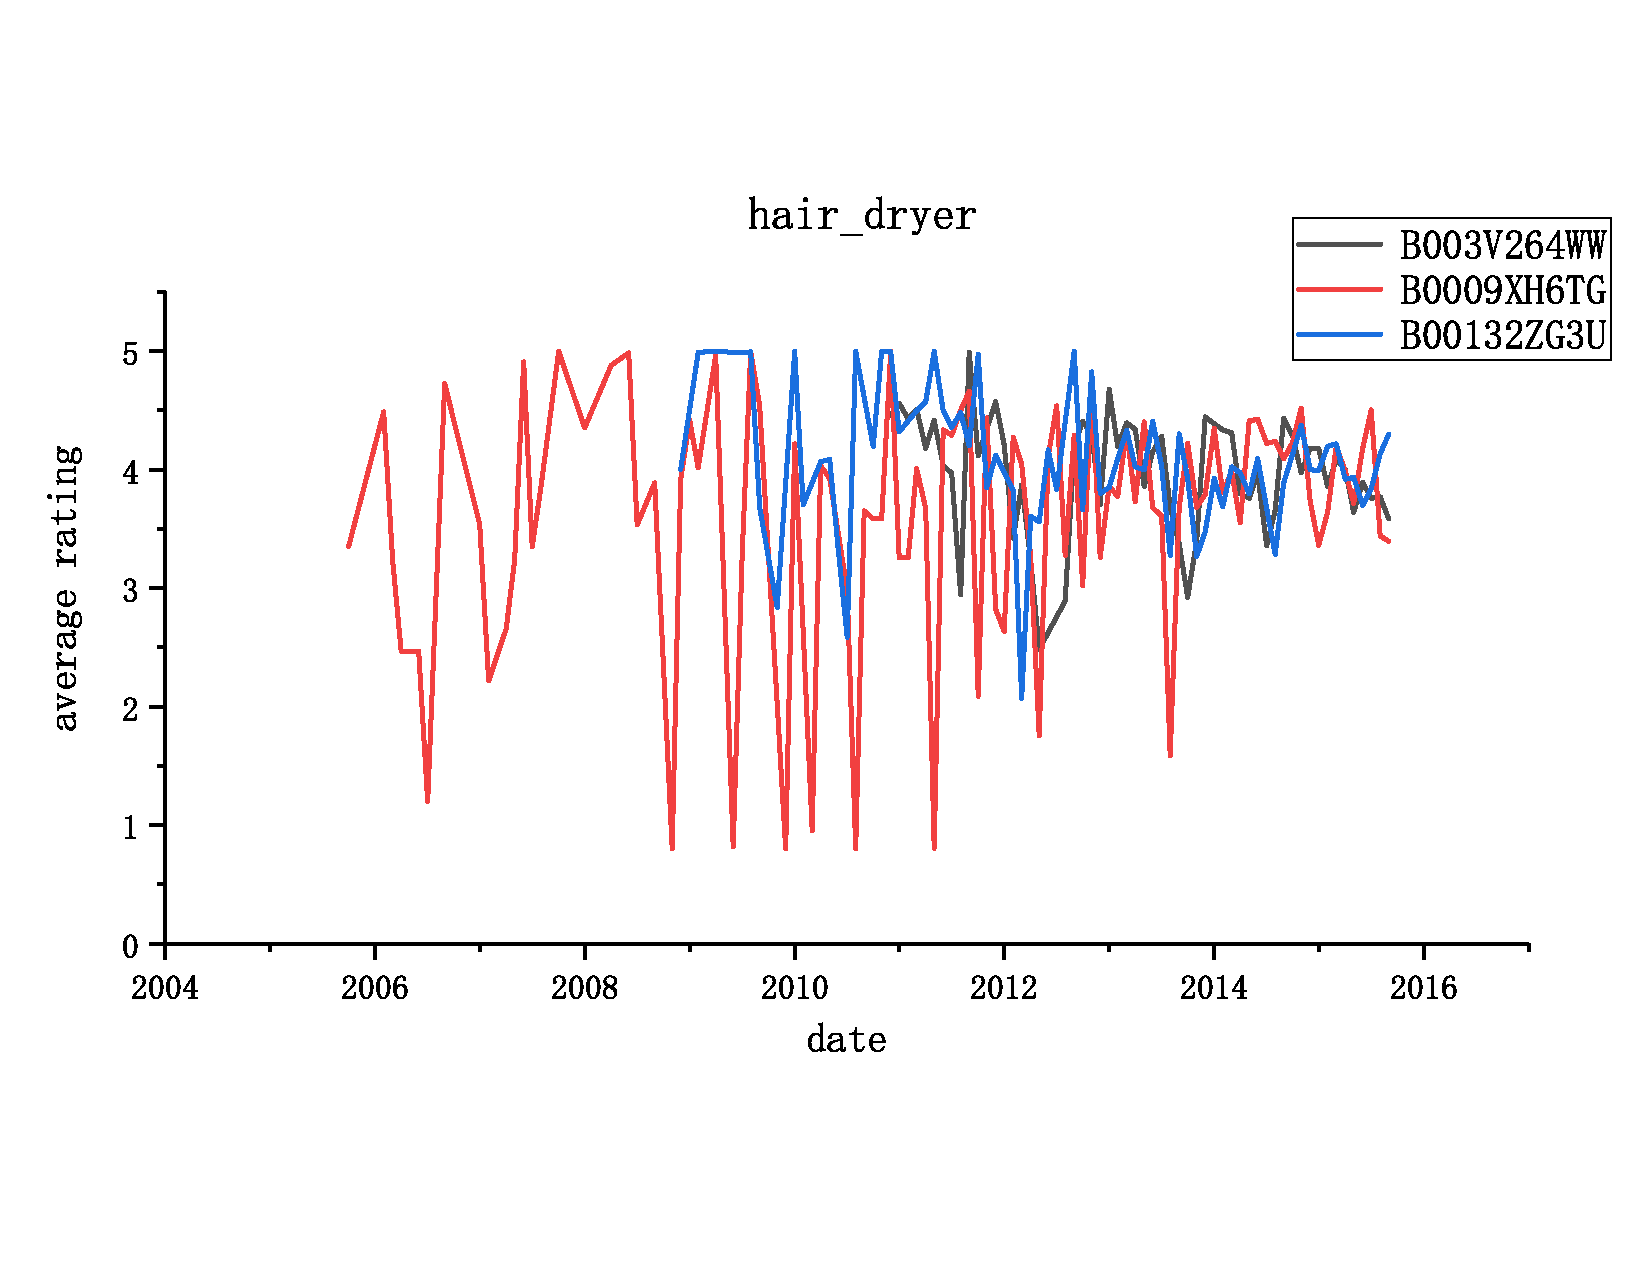
\includegraphics[width=15cm]{hair_dryer_ave_rating.eps}
		\caption{hair dryer average rating} \label{fig:hair dryer average rating}
	\end{figure}
	
	Combining the above figure, we find that the average score curves of these three products are very similar. In the early stages, product ratings fluctuated greatly because there were fewer customers. For example, the product B0009XH6TG (red line) has fluctuated between 1 and 5 stars in the early stage, the product B003V264WW (blue line) has fluctuated between 3 stars and 5 stars in the early stage, and the product B00132ZG3U (green line) has also fluctuated between 3 stars and 5 stars. In the later period, the scores of the three products stabilized at about 4 points, and the fluctuations did not exceed 0.5 points. It can be seen that the ratings of these three products in the later period are similar.
	
	Secondly, here is the chart of the top three microwave ovens\    (product\_id:B0055UBB40, B0058CLNBU,B0052G14E8):
	
	\begin{figure}[H]
		\small
		\centering
		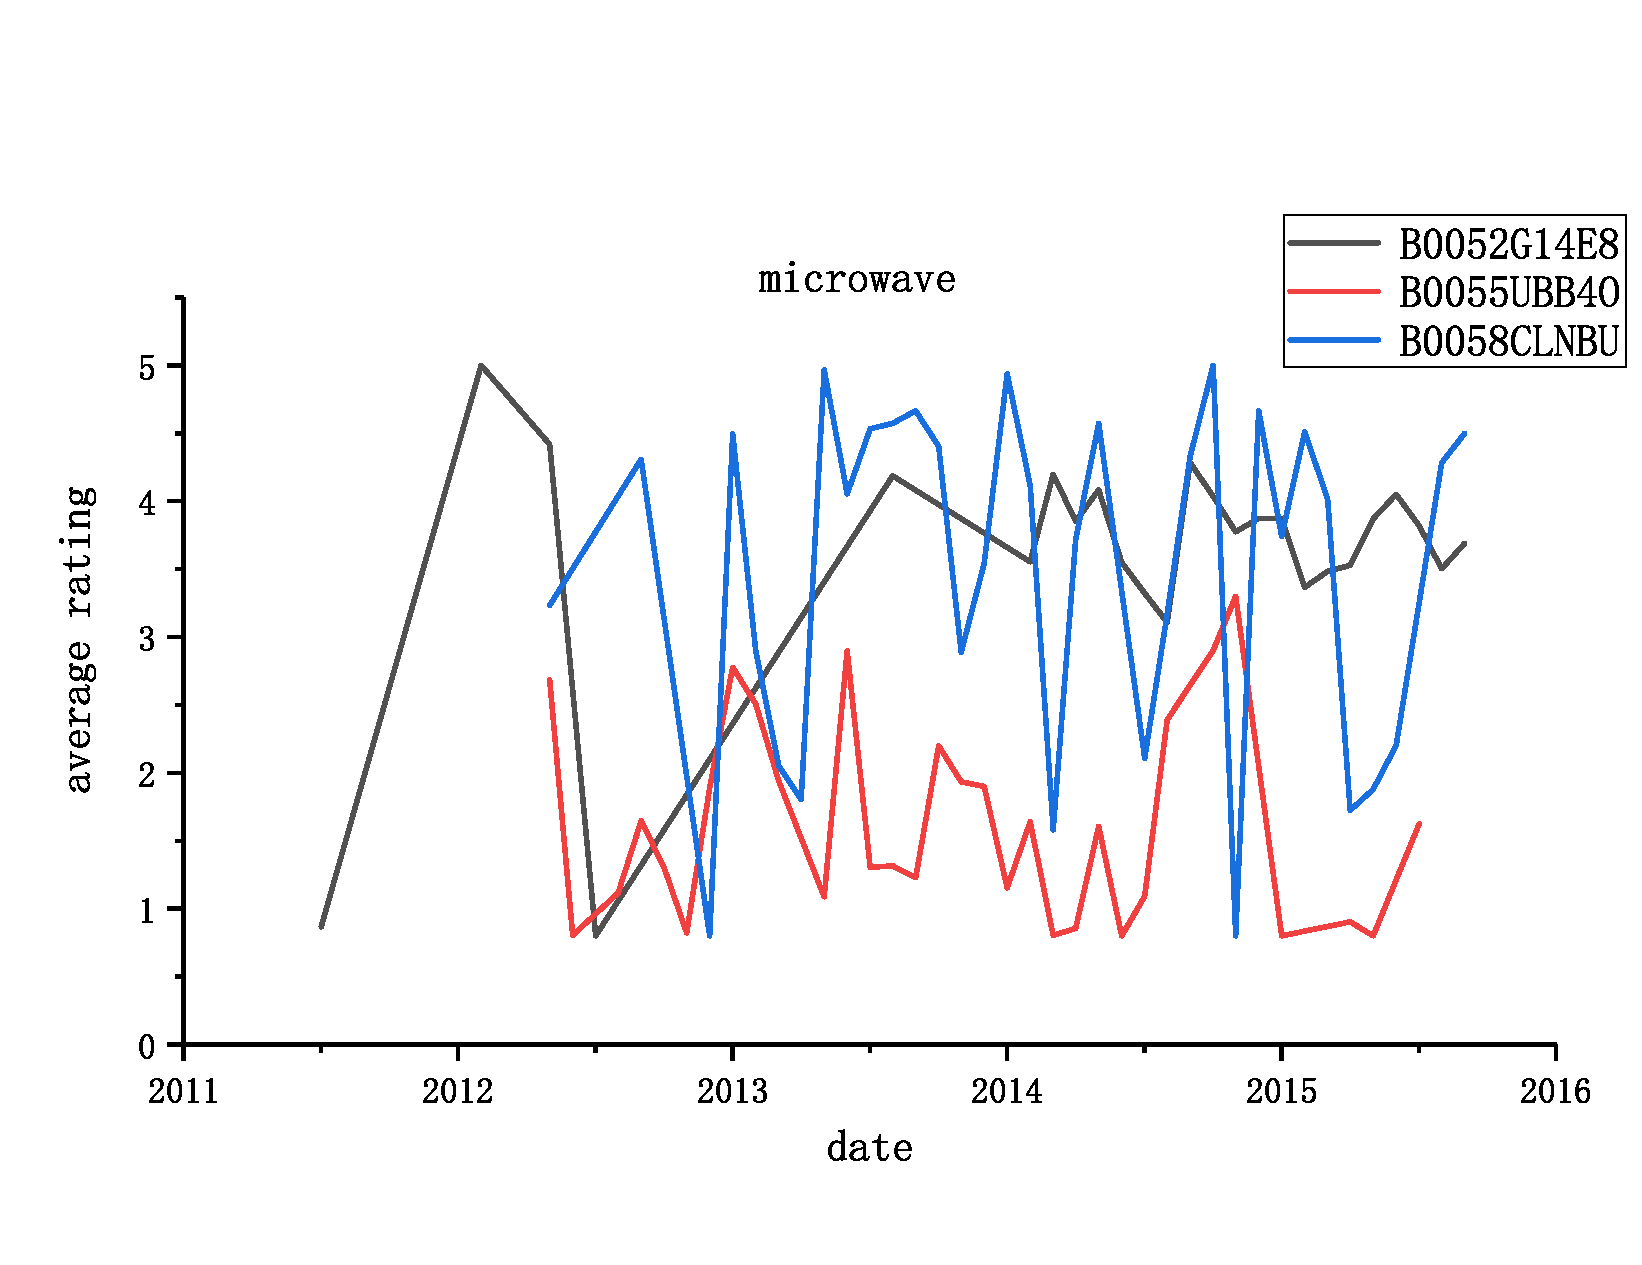
\includegraphics[width=15cm]{microwave_ave_rating.eps}
		\caption{microwave average rating} \label{fig:micorwave average rating}
	\end{figure}
	
	This picture is not different from the above picture, because the microwave oven has fewer reviews, the average rating fluctuates greatly. First of all, the product B0055UBB40 (red line) has been fluctuating between one star and three stars. Secondly, the product B0058CLNBU (blue line) has been fluctuating between one star and five stars, and the blue line has been almost above the red line. The final product B0052G14E8 (green line) fluctuated between one star and five stars in the early stage, and stabilized at about four stars in the later stage. It can be seen that the market feedback of product B0058CLNBU (blue line) and product B0052G14E8 (green line) is better than product B0055UBB40 (red line).
	
	Finally, the chart of the top three pacifiers is as follow:\ (product\_id:B003CK3LLDI, B0028IDXDS, B0045I6IA4):
	\begin{figure}[H]
		\small
		\centering
		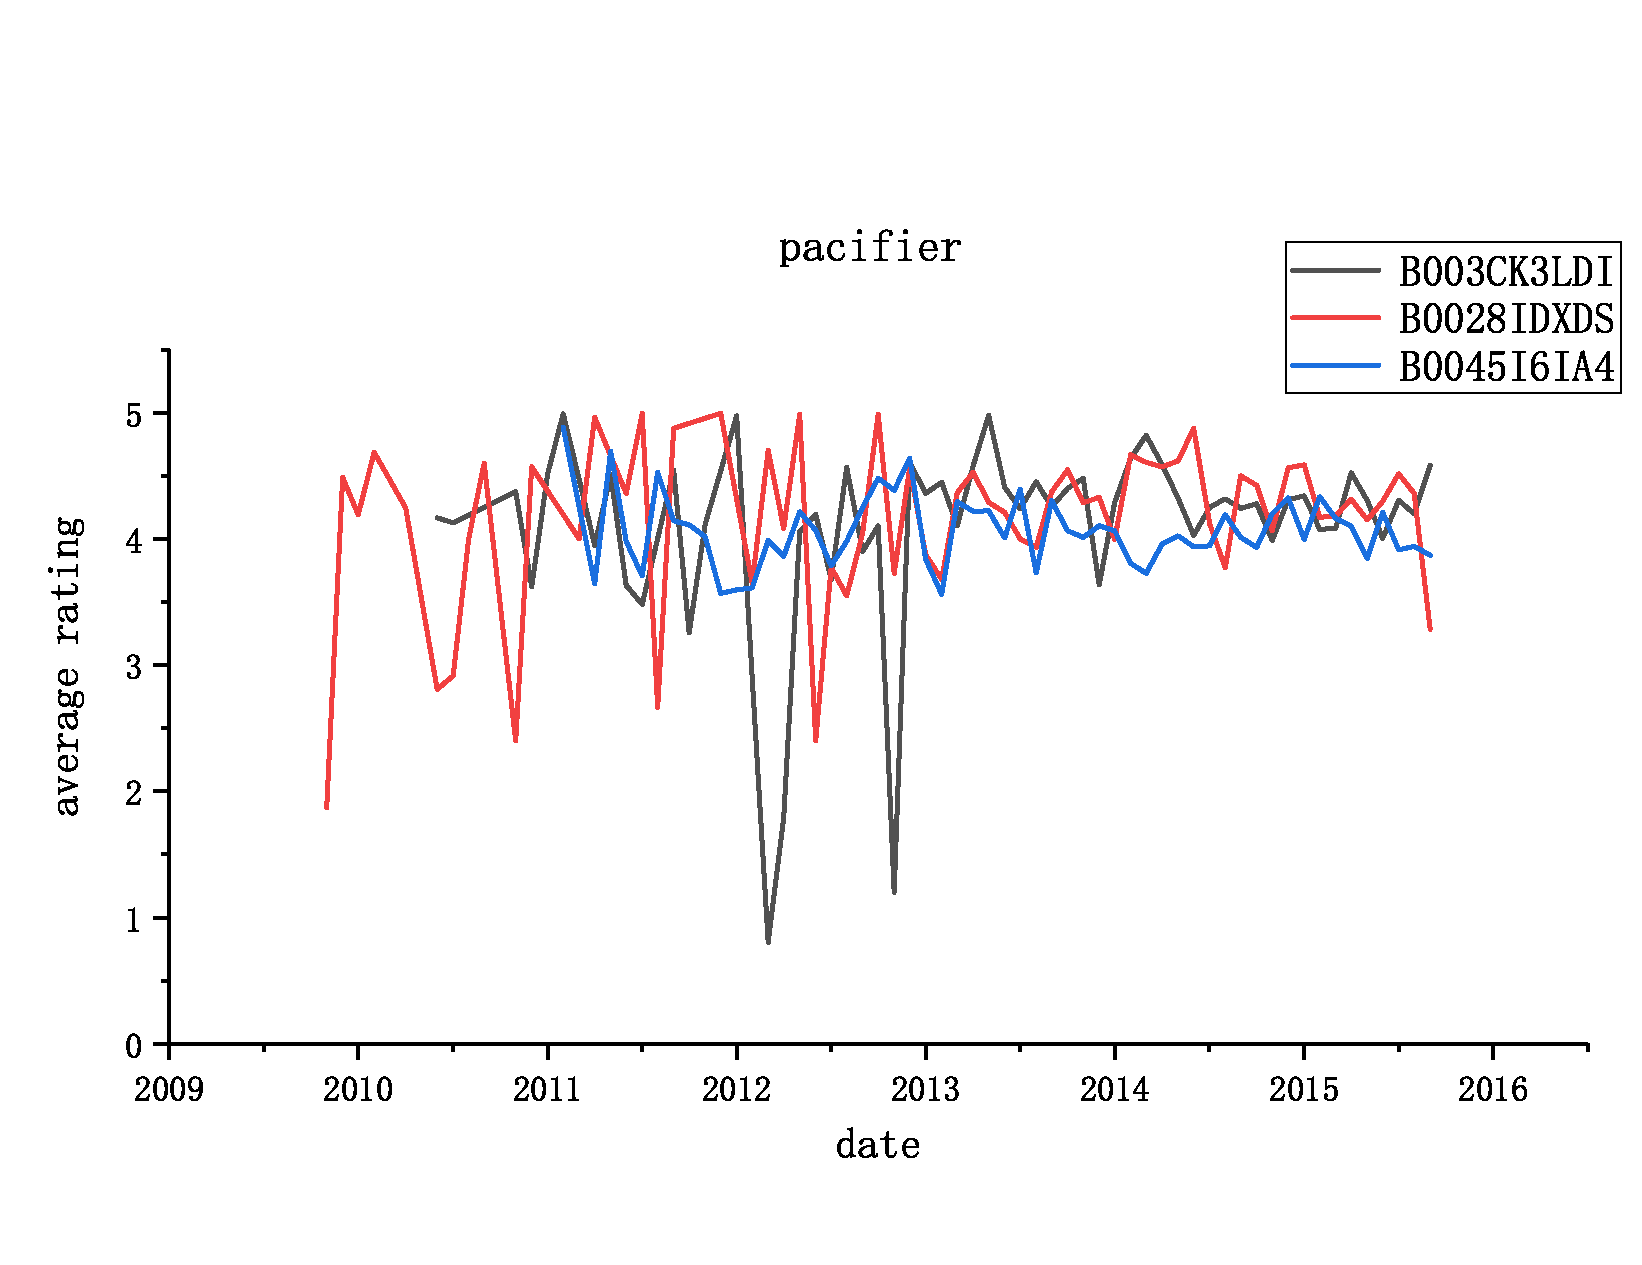
\includegraphics[width=15cm]{pacifier_ave_rating.eps}
		\caption{pacifier average rating} \label{fig:pacifier average rating}
	\end{figure}
	This picture is very similar to the picture about the hair dryer, both of which fluctuate in the early stage and stabilize in the later stage. In the later period, the three products were stable between four stars and 4.5 stars. In this regard, market feedback is better than hair dryers.
	
	
	
	
	\section{Summary}
	
	
	\section{Letter}
	
	
	\begin{thebibliography}{99}
		\bibitem{1} http://xiaohan2012.github.io/twitter-sent-dnn/
		\bibitem{2} Hu M , Liu B . Mining and summarizing customer reviews[C]// Proceedings of the Tenth ACM SIGKDD International Conference on Knowledge Discovery and Data Mining, Seattle, Washington, USA, August 22-25, 2004. ACM, 2004.
		
	\end{thebibliography}
	
	\begin{appendices}
		
		\section{First appendix}
		
		
		some more text \textcolor[rgb]{0.98,0.00,0.00}{\textbf{Input python source:}}
		\lstinputlisting[language=python]{./code/count_word_frequency.py}
		
	\end{appendices}
\end{document}

%%
%% This work consists of these files mcmthesis.dtx,
%%                                   figures/ and
%%                                   code/,
%% and the derived files             mcmthesis.cls,
%%                                   mcmthesis-demo.tex,
%%                                   README,
%%                                   LICENSE,
%%                                   mcmthesis.pdf and
%%                                   mcmthesis-demo.pdf.
%%
%% End of file `mcmthesis-demo.tex'.

